\begin{enumerate}[label=\thesubsection.\arabic*, ref=\thesubsection.\theenumi,itemsep=1.5em]

\item $PQ$ is a tangent to a circle with centre $O$ at the point $P$ on the circle. If $\triangle OPQ$ is an isosceles triangle, then find $\angle OQP$.
\hfill (CBSE~X~2021)
\\
\solution
From \eqref{eq:EE26BTECH11218-cb-tan-radius}, the direction $\vec{m}=\vec{Q}-\vec{P}$ of the tangent satisfies
\begin{align}
\brak{\vec{Q}-\vec{P}}^{\top}\brak{\vec{P}-\vec{O}} = 0 \implies \angle OPQ = 90^{\circ}
\end{align}
Hence, by Pythagoras,
\begin{align}
\norm{\vec{O}-\vec{Q}}^2 = \norm{\vec{O}-\vec{P}}^2 + \norm{\vec{P}-\vec{Q}}^2
\end{align}
so $OQ$ is strictly the longest side, and the equal sides of the isosceles triangle must be $OP$ and $PQ$. Since the shape is fixed up to rotation and scaling, take
\begin{align}
\vec{O} = \myvec{0 \\ 0}, \quad \vec{P} = \myvec{r \\ 0}, \quad \vec{m} = \myvec{0 \\ 1}, \quad \vec{Q} = \vec{P} + r\vec{m} = \myvec{r \\ r}
\end{align}
Substituting in \eqref{eq:EE26BTECH11218-cb-angle},
\begin{align}
\cos\angle OQP = \frac{\brak{\vec{O}-\vec{Q}}^{\top}\brak{\vec{P}-\vec{Q}}}{\norm{\vec{O}-\vec{Q}}\norm{\vec{P}-\vec{Q}}}
= \frac{\myvec{-r & -r}\myvec{0 \\ -r}}{r\sqrt{2}\cdot r} = \frac{1}{\sqrt{2}}
\end{align}
\begin{align}
\therefore \angle OQP = 45^{\circ}
\end{align}
The following code verifies this in \figref{fig:EE26BTECH11218-cb_q6}.
\begin{lstlisting}[frame=single, basicstyle=\rmfamily, escapeinside={(*@}{@*)}]
(*@\makebox[\dimexpr\linewidth-2\fboxsep-2\fboxrule\relax][c]{codes/cbXq6.py}@*)
\end{lstlisting}
\begin{figure}[H]
    \centering
    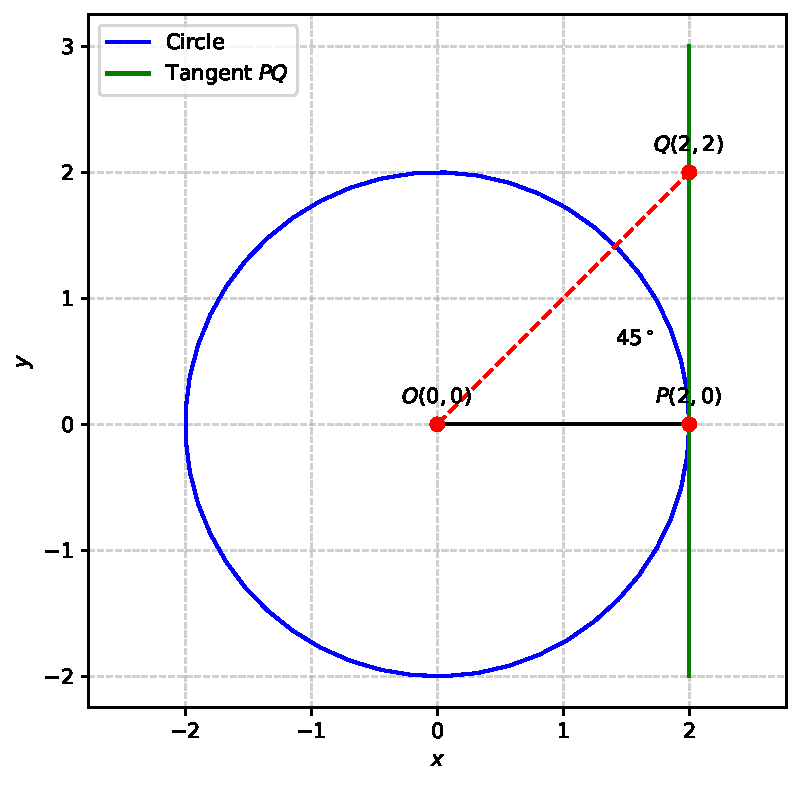
\includegraphics[width=0.70\linewidth]{figs/cbXq6.pdf}
    \caption{Tangent $PQ$ and the isosceles triangle $OPQ$ with $\angle OQP=45^{\circ}$}
    \label{fig:EE26BTECH11218-cb_q6}
\end{figure}
\item Two concentric circles have radii $10$ cm and $6$ cm. Find the length of the chord of the larger circle which touches the smaller circle.
\hfill (CBSE~X~2021)
\\
\solution
With the common centre at the origin, from \eqref{eq:EE26BTECH11218-cb-circle} the circles have
\begin{align}
\vec{V} = \vec{I}, \quad \vec{u} = \vec{0}, \quad f_1 = -100 \text{ (larger)}, \quad f_2 = -36 \text{ (smaller)}
\end{align}
Choose the axes so that the chord is the line $\vec{x} = \vec{h}+\kappa\vec{m}$ with
\begin{align}
\vec{h} = \myvec{6 \\ 0}, \quad \vec{m} = \myvec{0 \\ 1}, \quad \vec{m}^{\top}\vec{h}=0
\end{align}
For the smaller circle, $\vec{m}^{\top}\brak{\vec{V}\vec{h}+\vec{u}} = 0$ and $g\brak{\vec{h}} = \norm{\vec{h}}^2 - 36 = 0$, so \eqref{eq:EE26BTECH11218-cb-chord} gives $\Delta = 0$ and the line is tangent. For the larger circle, $g\brak{\vec{h}} = 36-100 = -64$, $\vec{m}^{\top}\vec{V}\vec{m} = 1$, so from \eqref{eq:EE26BTECH11218-cb-kappa}
\begin{align}
\kappa = \frac{0 \pm \sqrt{0 + 64}}{1} = \pm 8
\implies \vec{x}_{1,2} = \myvec{6 \\ \pm 8}
\end{align}
Hence the length of the chord, from \eqref{eq:EE26BTECH11218-cb-chord}, is
\begin{align}
\norm{\vec{x}_1-\vec{x}_2} = \abs{8-\brak{-8}}\norm{\vec{m}} = 16 \text{ cm}
\end{align}
The following code verifies this in \figref{fig:EE26BTECH11218-cb_q7}.
\begin{lstlisting}[frame=single, basicstyle=\rmfamily, escapeinside={(*@}{@*)}]
(*@\makebox[\dimexpr\linewidth-2\fboxsep-2\fboxrule\relax][c]{codes/cbXq7.py}@*)
\end{lstlisting}
\begin{figure}[H]
    \centering
    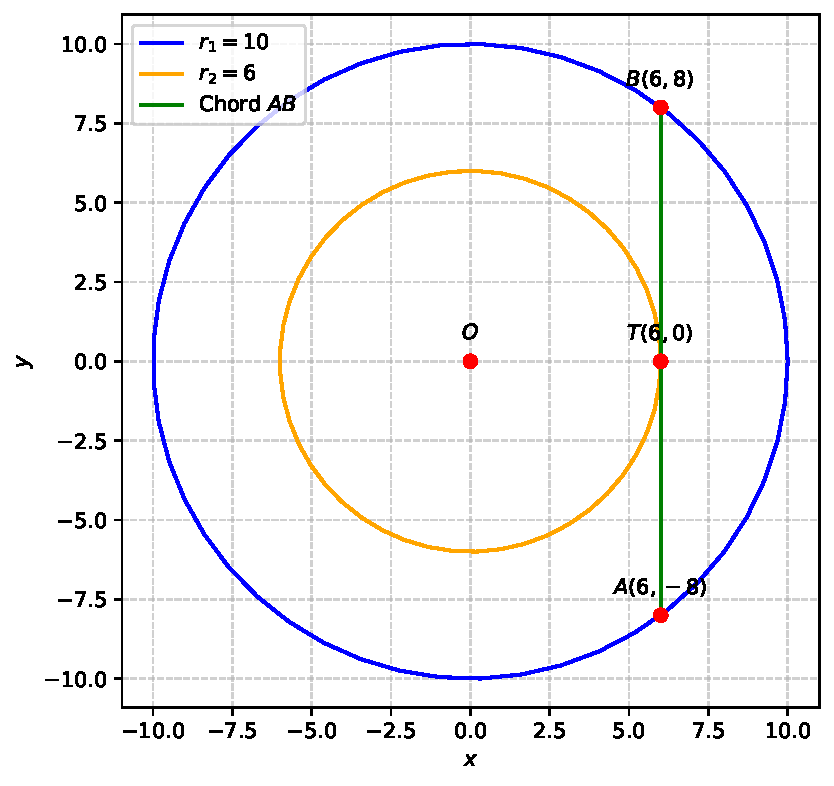
\includegraphics[width=0.70\linewidth]{figs/cbXq7.pdf}
    \caption{Chord of the larger circle touching the smaller circle}
    \label{fig:EE26BTECH11218-cb_q7}
\end{figure}
\item How many outcomes are possible when three dice are thrown together?
\hfill (CBSE~X~2021)
\\
\solution
For one die, the generating function of the outcomes is $x+x^2+\cdots+x^6$. For three dice, from \eqref{eq:EE26BTECH11218-cb-dice-count}, the number of outcomes with sum $n$ is the coefficient of $x^n$ in
\begin{align}
\brak{x+x^2+\cdots+x^6}^3 &= x^3 + 3x^4 + 6x^5 + 10x^6 + 15x^7 + 21x^8 \\
&\quad + 25x^9 + 27x^{10} + \cdots + x^{18}
\end{align}
and setting $x=1$ adds the counts of all sums,
\begin{align}
\brak{1+1+\cdots+1}^3 = 6^3 = 216
\end{align}
The following code verifies this in \figref{fig:EE26BTECH11218-cb_q16}.
\begin{lstlisting}[frame=single, basicstyle=\rmfamily, escapeinside={(*@}{@*)}]
(*@\makebox[\dimexpr\linewidth-2\fboxsep-2\fboxrule\relax][c]{codes/cbXq16.py}@*)
\end{lstlisting}
\begin{figure}[H]
    \centering
    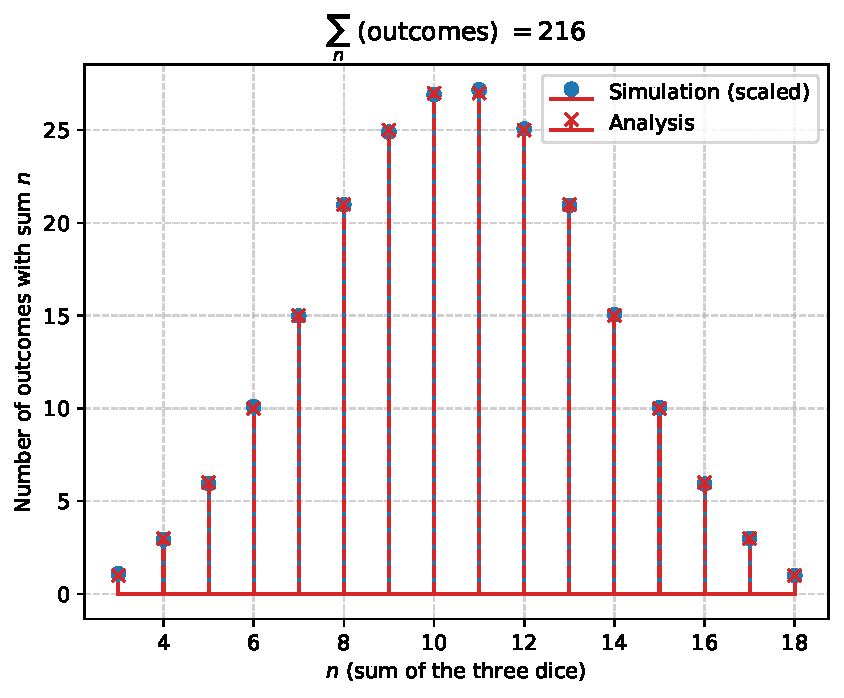
\includegraphics[width=0.70\linewidth]{figs/cbXq16.pdf}
    \caption{Number of outcomes for each sum of three dice: Simulation vs Analysis}
    \label{fig:EE26BTECH11218-cb_q16}
\end{figure}
\item The residents of a housing society decided to build two straight paths in the central park. Taking one corner of the park as origin and two mutually perpendicular lines as the axes, the paths are represented by $2x-3y=5$ and $-6x+9y=7$.
\hfill (CBSE~X~2021)

\begin{enumerate}[label=(\roman*), itemsep=0pt]
\item The two paths are
\begin{enumerate}[label=\alph*), itemsep=0pt]
    \begin{multicols}{2}
        \item intersecting
        \item overlapping
        \item parallel
        \item mutually perpendicular
    \end{multicols}
\end{enumerate}
\item Which of the following points lies on the line $2x-3y=5$?
\begin{enumerate}[label=\alph*), itemsep=0pt]
    \begin{multicols}{4}
        \item $\brak{-4,1}$
        \item $\brak{4,-1}$
        \item $\brak{4,1}$
        \item $\brak{-4,-1}$
    \end{multicols}
\end{enumerate}
\item If the line $-6x+9y=7$ intersects the $y$-axis at a point, its coordinates are
\begin{enumerate}[label=\alph*), itemsep=0pt]
    \begin{multicols}{4}
        \item $\brak{0,\frac{7}{9}}$
        \item $\brak{\frac{7}{9},0}$
        \item $\brak{-\frac{7}{6},0}$
        \item $\brak{0,-\frac{7}{6}}$
    \end{multicols}
\end{enumerate}
\item If a pair of equations $a_1x+b_1y+c_1=0$ and $a_2x+b_2y+c_2=0$ has a unique solution, then
\begin{enumerate}[label=\alph*), itemsep=0pt]
    \begin{multicols}{4}
        \item $\frac{a_1}{a_2}=\frac{b_1}{b_2}=\frac{c_1}{c_2}$
        \item $\frac{a_1}{a_2}\ne\frac{b_1}{b_2}$
        \item $\frac{a_1}{a_2}=\frac{b_1}{b_2}\ne\frac{c_1}{c_2}$
        \item $\frac{a_1}{a_2}\ne\frac{b_1}{b_2}\ne\frac{c_1}{c_2}$
    \end{multicols}
\end{enumerate}
\item If $\frac{a_1}{a_2}=\frac{b_1}{b_2}=\frac{c_1}{c_2}$, the two lines are
\begin{enumerate}[label=\alph*), itemsep=0pt]
    \begin{multicols}{4}
        \item parallel
        \item coincident
        \item intersecting
        \item perpendicular to each other
    \end{multicols}
\end{enumerate}
\end{enumerate}
\solution
The paths are the matrix equation \eqref{eq:EE26BTECH11218-cb-linsys} with
\begin{align}
\vec{A} = \myvec{2 & -3 \\ -6 & 9}, \quad \vec{b} = \myvec{5 \\ 7}
\end{align}
\textbf{(i)} The second row of $\vec{A}$ is $-3$ times the first, so $\mydet{\vec{A}} = 18-18 = 0$ and $\rank\brak{\vec{A}} = 1$. Applying $R_2 \to R_2+3R_1$ to the augmented matrix,
\begin{align}
\augvec{2}{1}{2 & -3 & 5 \\ -6 & 9 & 7} \xrightarrow{R_2 \to R_2+3R_1} \augvec{2}{1}{2 & -3 & 5 \\ 0 & 0 & 22}
\end{align}
so $\rank\brak{\vec{A}} = 1 < 2 = \rank\brak{\sbrak{\vec{A}\mid\vec{b}}}$. From \eqref{eq:EE26BTECH11218-cb-rank-cases} the system is inconsistent with parallel normals, so the paths are \textbf{parallel}: option (c). Their distance, writing the second line as $\vec{n}_1^{\top}\vec{x}=-\frac{7}{3}$ with $\vec{n}_1 = \myvec{2 \\ -3}$, is
\begin{align}
\frac{\abs{5-\brak{-\frac{7}{3}}}}{\norm{\vec{n}_1}} = \frac{22}{3\sqrt{13}} \approx 2.03
\end{align}
\textbf{(ii)} Evaluating $\vec{n}_1^{\top}\vec{x}_0$ for the four points gives $-11,\ 11,\ 5,\ -5$, and only $\brak{4,1}$ gives $5$: option (c).

\textbf{(iii)} On the $y$-axis $\vec{e}_1^{\top}\vec{x}=0$, so $9y=7$ and the point is $\brak{0,\frac{7}{9}}$: option (a).

\textbf{(iv)} A unique solution requires $\rank\brak{\vec{A}}=2$, i.e. $\mydet{\vec{A}} = a_1b_2-a_2b_1 \ne 0$. From \eqref{eq:EE26BTECH11218-cb-rank-cases} this is $\frac{a_1}{a_2}\ne\frac{b_1}{b_2}$: option (b).

\textbf{(v)} If the rows are proportional, $\rank\brak{\vec{A}} = \rank\brak{\sbrak{\vec{A}\mid\vec{b}}} = 1$, so the system has infinitely many solutions and the lines are \textbf{coincident}: option (b).

The following code verifies the results in \figref{fig:EE26BTECH11218-cb_q17}.
\begin{lstlisting}[frame=single, basicstyle=\rmfamily, escapeinside={(*@}{@*)}]
(*@\makebox[\dimexpr\linewidth-2\fboxsep-2\fboxrule\relax][c]{codes/cbXq17.py}@*)
\end{lstlisting}
\begin{figure}[H]
    \centering
    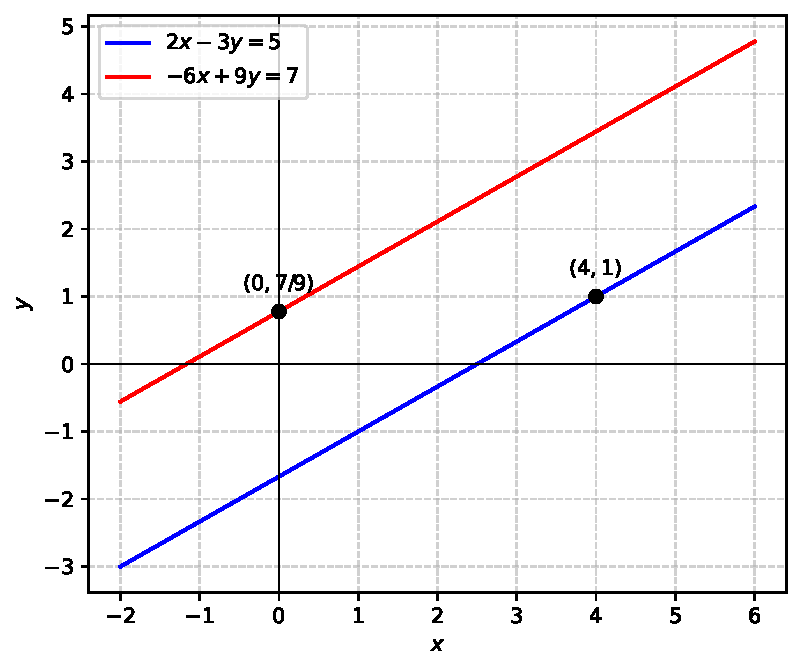
\includegraphics[width=0.70\linewidth]{figs/cbXq17.pdf}
    \caption{The parallel paths $2x-3y=5$ and $-6x+9y=7$}
    \label{fig:EE26BTECH11218-cb_q17}
\end{figure}
\item The time taken (in seconds) by a group of students to complete a race is recorded as follows.
\begin{center}
\begin{tabular}{|c|c|c|c|c|c|}
\hline
Time (s) & $0$--$20$ & $20$--$40$ & $40$--$60$ & $60$--$80$ & $80$--$100$ \\ \hline
Students & $1$ & $4$ & $3$ & $7$ & $5$ \\ \hline
\end{tabular}
\end{center}
\hfill (CBSE~X~2021)

\begin{enumerate}[label=(\roman*), itemsep=0pt]
\item The class mark of the modal class is
\begin{enumerate}[label=\alph*), itemsep=0pt]
    \begin{multicols}{4}
        \item $60$
        \item $70$
        \item $80$
        \item $140$
    \end{multicols}
\end{enumerate}
\item The mode of the given data is
\begin{enumerate}[label=\alph*), itemsep=0pt]
    \begin{multicols}{4}
        \item $70.33$
        \item $71.33$
        \item $72.33$
        \item $73.33$
    \end{multicols}
\end{enumerate}
\item The median class of the given data is
\begin{enumerate}[label=\alph*), itemsep=0pt]
    \begin{multicols}{4}
        \item $20$--$40$
        \item $40$--$60$
        \item $80$--$100$
        \item $60$--$80$
    \end{multicols}
\end{enumerate}
\item The sum of the lower limits of the median class and the modal class is
\begin{enumerate}[label=\alph*), itemsep=0pt]
    \begin{multicols}{4}
        \item $80$
        \item $140$
        \item $120$
        \item $100$
    \end{multicols}
\end{enumerate}
\item The median time (in seconds) of the given data is
\begin{enumerate}[label=\alph*), itemsep=0pt]
    \begin{multicols}{4}
        \item $65.7$
        \item $85.7$
        \item $45.7$
        \item $25.7$
    \end{multicols}
\end{enumerate}
\end{enumerate}
\solution
Here $h=20$, $N=\sum_i f_i = 20$, and the cumulative frequencies are
\begin{align}
F_i = 1,\ 5,\ 8,\ 15,\ 20
\end{align}
\textbf{(i)} The largest frequency is $7$, so the modal class is $60$--$80$ with class mark $\frac{60+80}{2}=70$: option (b).

\textbf{(ii)} With $l=60$, $f_0=3$, $f_1=7$, $f_2=5$, the two lines of the histogram construction pass through
\begin{align}
\vec{A}_1 = \myvec{60 \\ 3},\ \vec{B}_1 = \myvec{80 \\ 7}, \qquad \vec{A}_2 = \myvec{60 \\ 7},\ \vec{B}_2 = \myvec{80 \\ 5}
\end{align}
The direction vectors are $\vec{m}_1 = \myvec{20 \\ 4}$, $\vec{m}_2 = \myvec{20 \\ -2}$, with normals obtained by a $90^{\circ}$ rotation, $\vec{n}_i = \myvec{0 & 1 \\ -1 & 0}\vec{m}_i$, so that
\begin{align}
\myvec{4 & -20 \\ -2 & -20}\vec{x} = \myvec{\vec{n}_1^{\top}\vec{A}_1 \\ \vec{n}_2^{\top}\vec{A}_2} = \myvec{180 \\ -260}
\implies \vec{x} = \myvec{73.33 \\ 5.67}
\end{align}
Its abscissa is the mode, which agrees with \eqref{eq:EE26BTECH11218-cb-mode}
\begin{align}
60 + \frac{7-3}{14-3-5}\times 20 = 73.33
\end{align}
option (d).

\textbf{(iii)} Since $\frac{N}{2}=10$ and $F_3 = 8 < 10 \le 15 = F_4$, the median class is $60$--$80$: option (d).

\textbf{(iv)} The lower limits of both classes are $60$, so the sum is $120$: option (c).

\textbf{(v)} From \eqref{eq:EE26BTECH11218-cb-median}, with $l=60$, $F_{k-1}=8$, $f_k=7$,
\begin{align}
\text{Median} = 60 + \frac{10-8}{7}\times 20 = 60+\frac{40}{7} \approx 65.7
\end{align}
option (a). The following code verifies the mode as a line intersection and the median as the root of the ogive in \figref{fig:EE26BTECH11218-cb_q19}.
\begin{lstlisting}[frame=single, basicstyle=\rmfamily, escapeinside={(*@}{@*)}]
(*@\makebox[\dimexpr\linewidth-2\fboxsep-2\fboxrule\relax][c]{codes/cbXq19.py}@*)
\end{lstlisting}
\begin{figure}[H]
    \centering
    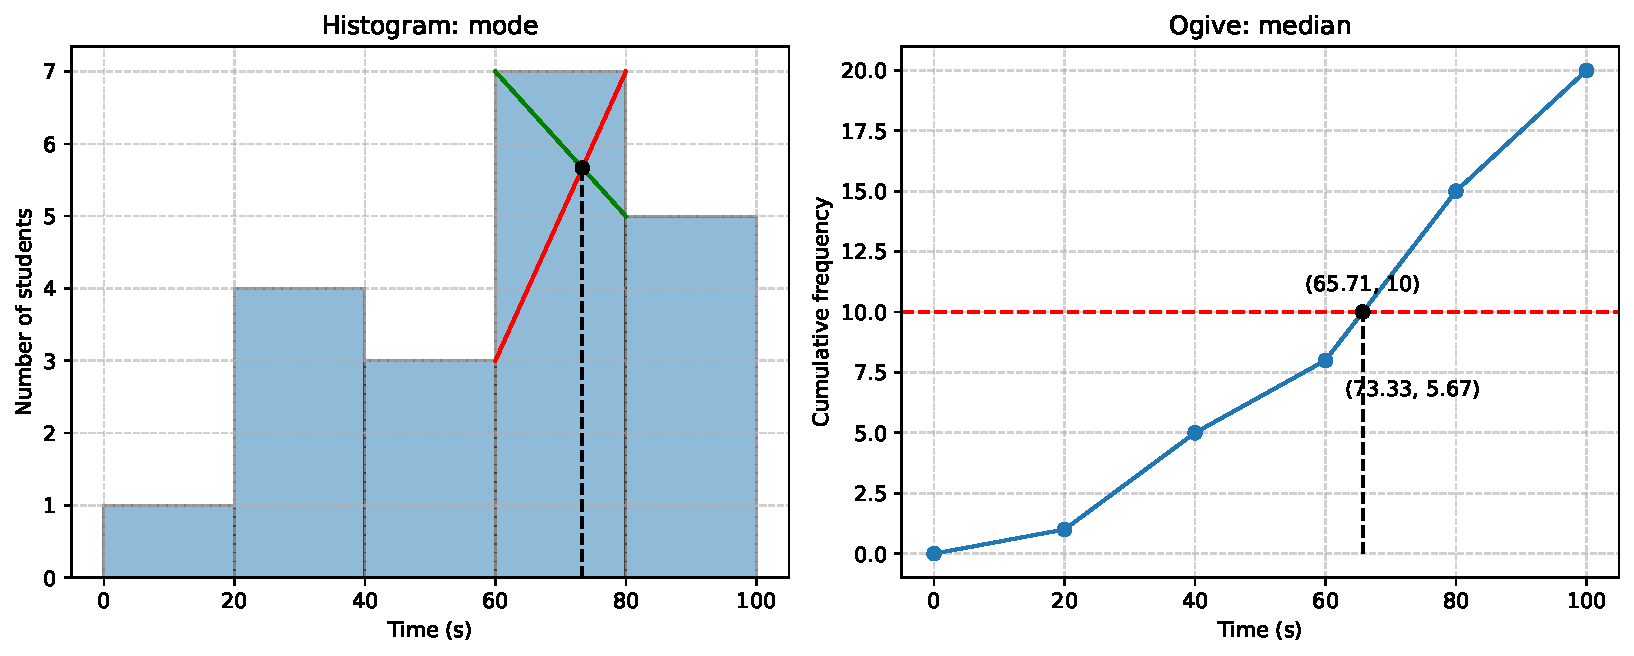
\includegraphics[width=0.95\linewidth]{figs/cbXq19.pdf}
    \caption{Histogram construction for the mode and ogive for the median}
    \label{fig:EE26BTECH11218-cb_q19}
\end{figure}
\item Twenty identical cards are numbered $1$ to $20$ and placed in a box. One card is drawn at random.
\hfill (CBSE~X~2021)

\begin{enumerate}[label=(\roman*), itemsep=0pt]
\item The probability that the number on the card is an odd prime number is
\begin{enumerate}[label=\alph*), itemsep=0pt]
    \begin{multicols}{4}
        \item $\frac{3}{5}$
        \item $\frac{2}{5}$
        \item $\frac{9}{20}$
        \item $\frac{7}{20}$
    \end{multicols}
\end{enumerate}
\item The probability that the number on the card is a composite number is
\begin{enumerate}[label=\alph*), itemsep=0pt]
    \begin{multicols}{4}
        \item $\frac{11}{20}$
        \item $\frac{3}{5}$
        \item $\frac{4}{5}$
        \item $\frac{1}{2}$
    \end{multicols}
\end{enumerate}
\item The probability that the number on the card is a multiple of $3$, $6$ and $9$ is
\begin{enumerate}[label=\alph*), itemsep=0pt]
    \begin{multicols}{4}
        \item $\frac{1}{20}$
        \item $\frac{1}{10}$
        \item $\frac{3}{20}$
        \item $0$
    \end{multicols}
\end{enumerate}
\item The probability that the number on the card is a multiple of $3$ and $7$ is
\begin{enumerate}[label=\alph*), itemsep=0pt]
    \begin{multicols}{4}
        \item $\frac{3}{10}$
        \item $\frac{1}{10}$
        \item $0$
        \item $\frac{2}{5}$
    \end{multicols}
\end{enumerate}
\item If all cards with odd numbers are removed and one card is drawn from the rest, the probability of a prime number is
\begin{enumerate}[label=\alph*), itemsep=0pt]
    \begin{multicols}{4}
        \item $\frac{1}{20}$
        \item $\frac{1}{10}$
        \item $0$
        \item $\frac{1}{5}$
    \end{multicols}
\end{enumerate}
\end{enumerate}
\solution
Let $\Omega = \cbrak{1,2,\dots,20}$ with $p_X\brak{n} = \frac{1}{20}$ and use \eqref{eq:EE26BTECH11218-cb-prob}. The primes in $\Omega$ are
\begin{align}
\cbrak{2,3,5,7,11,13,17,19}, \quad \abs{\cbrak{\text{primes}}} = 8
\end{align}
\textbf{(i)} Removing $2$ leaves $7$ odd primes, so $\pr{\text{odd prime}} = \frac{7}{20}$: option (d).

\textbf{(ii)} Neither $1$ nor a prime is composite, so $\abs{\cbrak{\text{composite}}} = 20-1-8 = 11$ and $\pr{\text{composite}}=\frac{11}{20}$: option (a).

\textbf{(iii)} A multiple of $3$, $6$ and $9$ is a multiple of $\operatorname{lcm}\brak{3,6,9}=18$. From \eqref{eq:EE26BTECH11218-cb-lcm}, the count is $\left\lfloor\frac{20}{18}\right\rfloor = 1$, so the probability is $\frac{1}{20}$: option (a).

\textbf{(iv)} $\operatorname{lcm}\brak{3,7}=21>20$, so the count is $\left\lfloor\frac{20}{21}\right\rfloor = 0$ and the probability is $0$: option (c).

\textbf{(v)} Let $E$ be the event ``even number'' and $S$ the event ``prime''. Then $\pr{E}=\frac{10}{20}$ and $SE=\cbrak{2}$, so
\begin{align}
\pr{S\mid E} = \frac{\pr{SE}}{\pr{E}} = \frac{1/20}{1/2} = \frac{1}{10}
\end{align}
option (b). The following code verifies these in \figref{fig:EE26BTECH11218-cb_q20}.
\begin{lstlisting}[frame=single, basicstyle=\rmfamily, escapeinside={(*@}{@*)}]
(*@\makebox[\dimexpr\linewidth-2\fboxsep-2\fboxrule\relax][c]{codes/cbXq20.py}@*)
\end{lstlisting}
\begin{figure}[H]
    \centering
    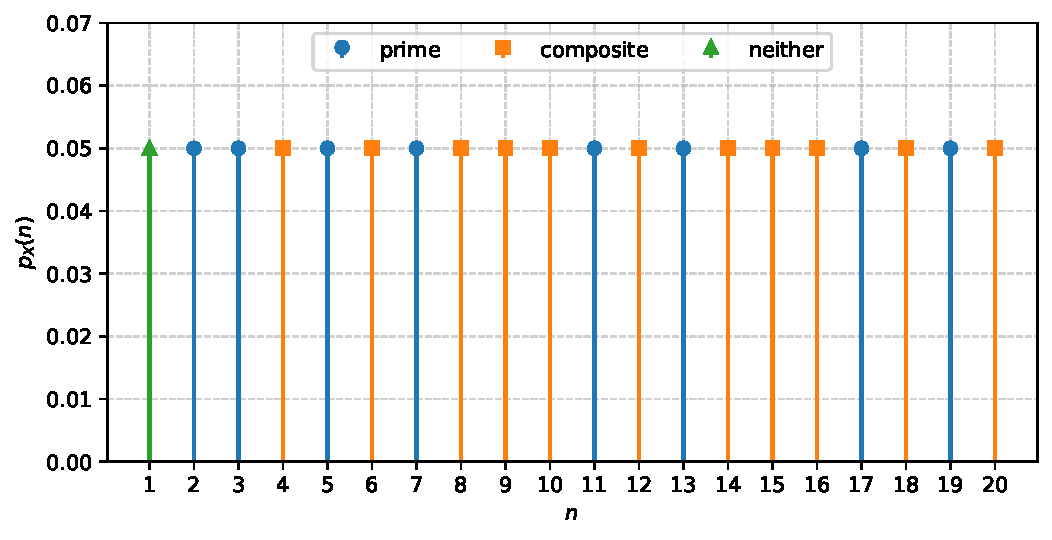
\includegraphics[width=0.70\linewidth]{figs/cbXq20.pdf}
    \caption{PMF of the card drawn, grouped as prime, composite and neither}
    \label{fig:EE26BTECH11218-cb_q20}
\end{figure}
\item Find the value of $k$ for which the system of equations $x+2y=5$ and $3x+ky+15=0$ has no solution.
\hfill (CBSE~X~2021)
\\
\solution
From \eqref{eq:EE26BTECH11218-cb-linsys},
\begin{align}
\myvec{1 & 2 \\ 3 & k}\myvec{x \\ y} = \myvec{5 \\ -15}
\end{align}
Applying Gaussian elimination to the augmented matrix,
\begin{align}
\augvec{2}{1}{1 & 2 & 5 \\ 3 & k & -15} \xrightarrow{R_2 \to R_2-3R_1} \augvec{2}{1}{1 & 2 & 5 \\ 0 & k-6 & -30}
\end{align}
If $k\ne6$, then $\rank\brak{\vec{A}}=2$ and the solution is unique. If $k=6$, then $\rank\brak{\vec{A}}=1$ while the last row of the augmented matrix is $\myvec{0 & 0 & -30}$, so $\rank\brak{\sbrak{\vec{A}\mid\vec{b}}}=2$. From \eqref{eq:EE26BTECH11218-cb-rank-cases},
\begin{align}
\rank\brak{\vec{A}} < \rank\brak{\sbrak{\vec{A}\mid\vec{b}}} \implies k = 6
\end{align}
This agrees with $\frac{1}{3}=\frac{2}{k}\ne\frac{-5}{15}$ at $k=6$. The following code verifies this in \figref{fig:EE26BTECH11218-cb_q22}.
\begin{lstlisting}[frame=single, basicstyle=\rmfamily, escapeinside={(*@}{@*)}]
(*@\makebox[\dimexpr\linewidth-2\fboxsep-2\fboxrule\relax][c]{codes/cbXq22.py}@*)
\end{lstlisting}
\begin{figure}[H]
    \centering
    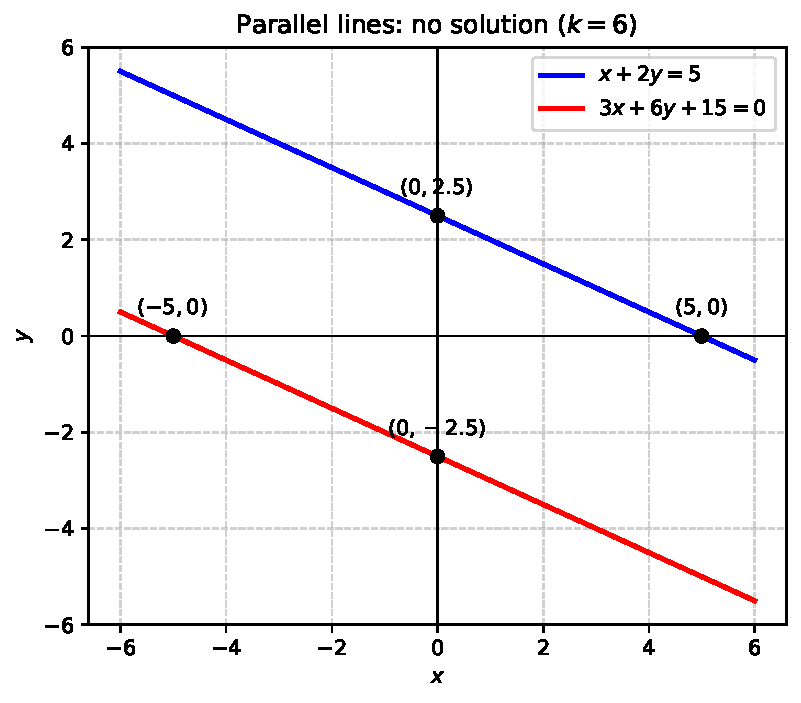
\includegraphics[width=0.70\linewidth]{figs/cbXq22.pdf}
    \caption{Parallel lines $x+2y=5$ and $3x+6y+15=0$ ($k=6$): no solution}
    \label{fig:EE26BTECH11218-cb_q22}
\end{figure}
\item $ABC$ is a right triangle, right-angled at $B$, with $BC=6$ cm and $AB=8$ cm. A circle with centre $O$ and radius $r$ cm is inscribed in $\triangle ABC$. Find the value of $r$.
\hfill (CBSE~X~2021)
\\
\solution
Taking $B$ as the origin with $BC$ and $BA$ along the axes,
\begin{align}
\vec{A} = \myvec{0 \\ 8}, \quad \vec{B} = \myvec{0 \\ 0}, \quad \vec{C} = \myvec{6 \\ 0}
\end{align}
The sides are $a=BC=6$, $c=AB=8$ and $b=CA=\norm{\vec{C}-\vec{A}}=10$. From \eqref{eq:EE26BTECH11218-cb-incircle},
\begin{align}
\vec{I} = \frac{6\myvec{0 \\ 8} + 10\myvec{0 \\ 0} + 8\myvec{6 \\ 0}}{24} = \myvec{2 \\ 2}, \qquad
r = \frac{\Delta}{s} = \frac{\frac{1}{2}\cdot6\cdot8}{12} = 2
\end{align}
Using the linear system \eqref{eq:EE26BTECH11218-cb-incircle-sys} with the inward unit normals of $AB$, $BC$ and $CA$ ($4x+3y=24$),
\begin{align}
\myvec{1 & 0 & -1 \\ 0 & 1 & -1 \\ -0.8 & -0.6 & -1}\myvec{x \\ y \\ r} = \myvec{0 \\ 0 \\ -4.8}
\implies \myvec{x \\ y \\ r} = \myvec{2 \\ 2 \\ 2}
\end{align}
Also, from \eqref{eq:EE26BTECH11218-cb-incircle-right}, $r = \frac{6+8-10}{2} = 2$.
\begin{align}
\therefore r = 2 \text{ cm}
\end{align}
The points of contact are $\vec{P}=\myvec{0 \\ 2}$, $\vec{Q}=\myvec{2 \\ 0}$ and $\vec{R}=\myvec{3.6 \\ 3.2}$. The following code verifies this in \figref{fig:EE26BTECH11218-cb_q25}.
\begin{lstlisting}[frame=single, basicstyle=\rmfamily, escapeinside={(*@}{@*)}]
(*@\makebox[\dimexpr\linewidth-2\fboxsep-2\fboxrule\relax][c]{codes/cbXq25.py}@*)
\end{lstlisting}
\begin{figure}[H]
    \centering
    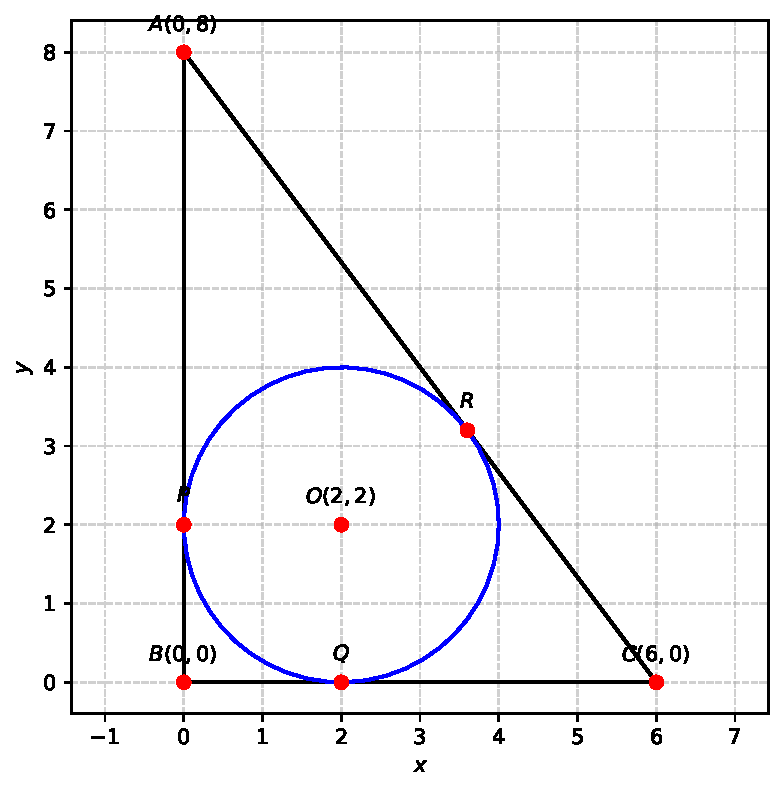
\includegraphics[width=0.70\linewidth]{figs/cbXq25.pdf}
    \caption{Incircle of the right triangle $ABC$ with $r=2$}
    \label{fig:EE26BTECH11218-cb_q25}
\end{figure}
\item Divide the polynomial $f\brak{x} = 5x^3+10x^2-30x-15$ by the polynomial $g\brak{x} = x^2+1+x$ and hence find the quotient and the remainder.
\hfill (CBSE~X~2021)
\\
\solution
From \eqref{eq:EE26BTECH11218-cb-division}, let $q\brak{x}=q_1x+q_0$ and $r\brak{x}=r_1x+r_0$. Then
\begin{align}
q\brak{x}g\brak{x} + r\brak{x} = q_1x^3 + \brak{q_1+q_0}x^2 + \brak{q_1+q_0+r_1}x + \brak{q_0+r_0}
\end{align}
Comparing coefficients with $f\brak{x}$ gives the matrix equation
\begin{align}
\myvec{1 & 0 & 0 & 0 \\ 1 & 1 & 0 & 0 \\ 1 & 1 & 1 & 0 \\ 0 & 1 & 0 & 1}\myvec{q_1 \\ q_0 \\ r_1 \\ r_0} = \myvec{5 \\ 10 \\ -30 \\ -15}
\implies \myvec{q_1 \\ q_0 \\ r_1 \\ r_0} = \myvec{5 \\ 5 \\ -40 \\ -20}
\end{align}
Verifying the remainder with \eqref{eq:EE26BTECH11218-cb-remainder}: the roots of $g$ are $\omega,\omega^2$ with $\omega^3=1$ and $\omega^2=-1-\omega$, so
\begin{align}
f\brak{\omega} = 5 + 10\omega^2 - 30\omega - 15 = -20-40\omega = r\brak{\omega}
\end{align}
and similarly for $\omega^2$, which gives $r\brak{x}=-40x-20$.
\begin{align}
\therefore q\brak{x} = 5x+5, \quad r\brak{x} = -40x-20
\end{align}
The following code verifies this in \figref{fig:EE26BTECH11218-cb_q27}.
\begin{lstlisting}[frame=single, basicstyle=\rmfamily, escapeinside={(*@}{@*)}]
(*@\makebox[\dimexpr\linewidth-2\fboxsep-2\fboxrule\relax][c]{codes/cbXq27.py}@*)
\end{lstlisting}
\begin{figure}[H]
    \centering
    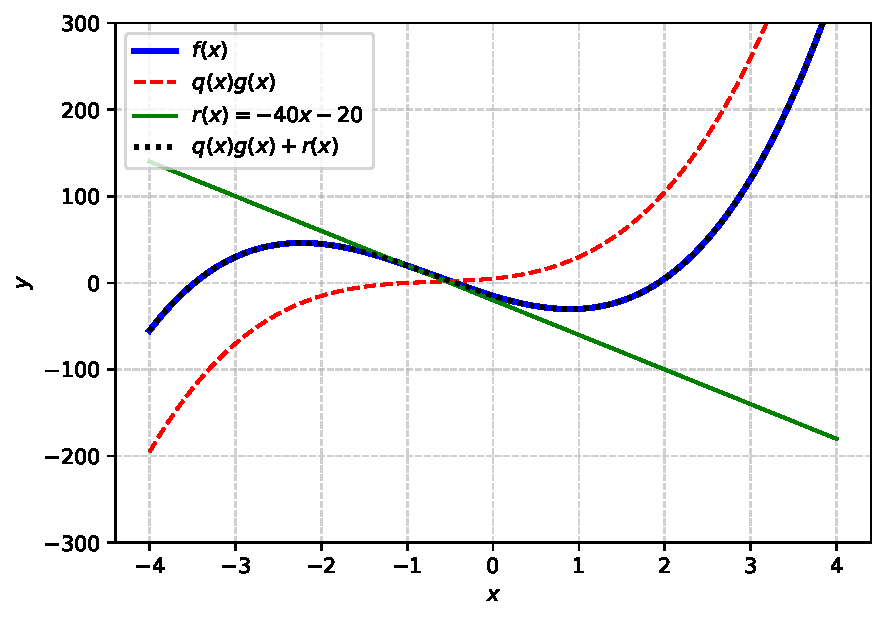
\includegraphics[width=0.70\linewidth]{figs/cbXq27.pdf}
    \caption{$f\brak{x}$ and $q\brak{x}g\brak{x}+r\brak{x}$ coincide}
    \label{fig:EE26BTECH11218-cb_q27}
\end{figure}
\item Water is being pumped out through a circular pipe whose internal diameter is $8$ cm. If the rate of flow of water is $80$ cm/s, how many litres of water are pumped out through this pipe in one hour?
\hfill (CBSE~X~2021)
\\
\solution
Here $R=4$ cm, $v=80$ cm/s and $T=3600$ s. From \eqref{eq:EE26BTECH11218-cb-flux},
\begin{align}
Q &= \int_0^{2\pi}\int_0^4 80\rho\,d\rho\,d\theta = 80\cdot2\pi\cdot8 = 1280\pi \text{ cm}^3/\text{s} \\
V &= \int_0^{3600} Q\,dt = 1280\pi\times3600 = 4608000\pi \text{ cm}^3
\end{align}
Since $1\text{ L}=1000\text{ cm}^3$,
\begin{align}
V = 4608\pi \text{ L} \approx 14476.46 \text{ L}
\end{align}
(with $\pi=\frac{22}{7}$, $V \approx 14482.29$ L). The following code verifies this in \figref{fig:EE26BTECH11218-cb_q34}.
\begin{lstlisting}[frame=single, basicstyle=\rmfamily, escapeinside={(*@}{@*)}]
(*@\makebox[\dimexpr\linewidth-2\fboxsep-2\fboxrule\relax][c]{codes/cbXq34.py}@*)
\end{lstlisting}
\begin{figure}[H]
    \centering
    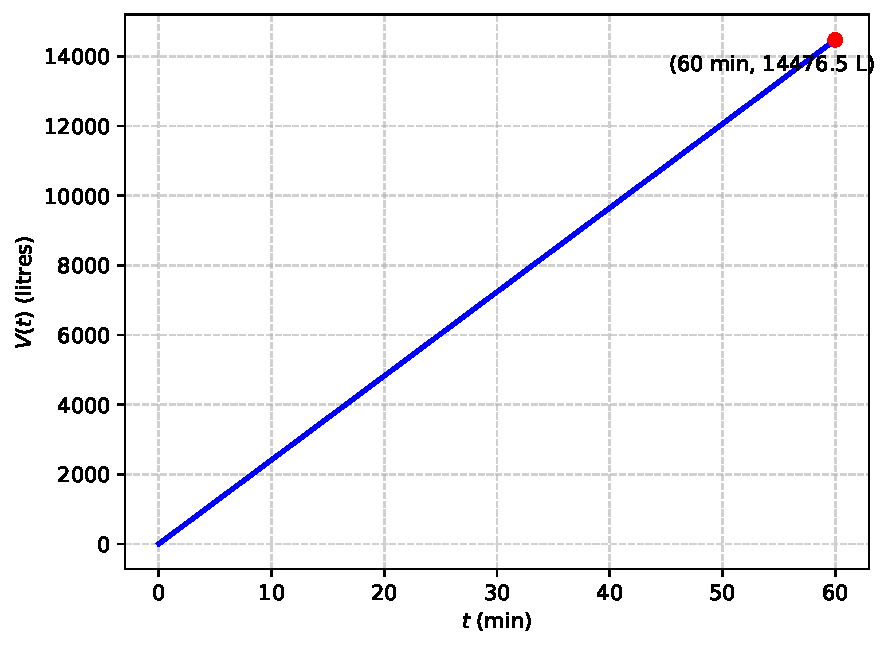
\includegraphics[width=0.70\linewidth]{figs/cbXq34.pdf}
    \caption{Volume pumped out versus time}
    \label{fig:EE26BTECH11218-cb_q34}
\end{figure}
\item A man on the top of a vertical tower observes a car moving at a uniform speed coming directly towards it. If it takes $18$ minutes for the angle of depression to change from $30^{\circ}$ to $60^{\circ}$, how soon after this will the car reach the tower?
\hfill (CBSE~X~2021)
\\
\solution
Let the tower have height $h$ and let $x\brak{t}$ be the horizontal distance of the car from its foot, with $t=0$ at the first observation. From \eqref{eq:EE26BTECH11218-cb-depression},
\begin{align}
x\brak{0} = h\cot30^{\circ} = \sqrt{3}h, \qquad x\brak{18} = h\cot60^{\circ} = \frac{h}{\sqrt{3}}
\end{align}
Using \eqref{eq:EE26BTECH11218-cb-uniform} and \eqref{eq:EE26BTECH11218-cb-uniform-sys} with $t_1=0$, $t_2=18$,
\begin{align}
\myvec{1 & 0 \\ 1 & -18}\myvec{x_0 \\ v} = \myvec{\sqrt{3}h \\ \frac{h}{\sqrt{3}}}
\implies x_0 = \sqrt{3}h, \quad v = \frac{1}{18}\brak{\sqrt{3}-\frac{1}{\sqrt{3}}}h = \frac{h}{9\sqrt{3}}
\end{align}
The car reaches the tower when $x\brak{t}=0$, that is after a further time
\begin{align}
t^{*} = \frac{x\brak{18}}{v} = \frac{h/\sqrt{3}}{h/\brak{9\sqrt{3}}} = 9 \text{ minutes}
\end{align}
which is independent of $h$. The following code verifies this in \figref{fig:EE26BTECH11218-cb_q35}.
\begin{lstlisting}[frame=single, basicstyle=\rmfamily, escapeinside={(*@}{@*)}]
(*@\makebox[\dimexpr\linewidth-2\fboxsep-2\fboxrule\relax][c]{codes/cbXq35.py}@*)
\end{lstlisting}
\begin{figure}[H]
    \centering
    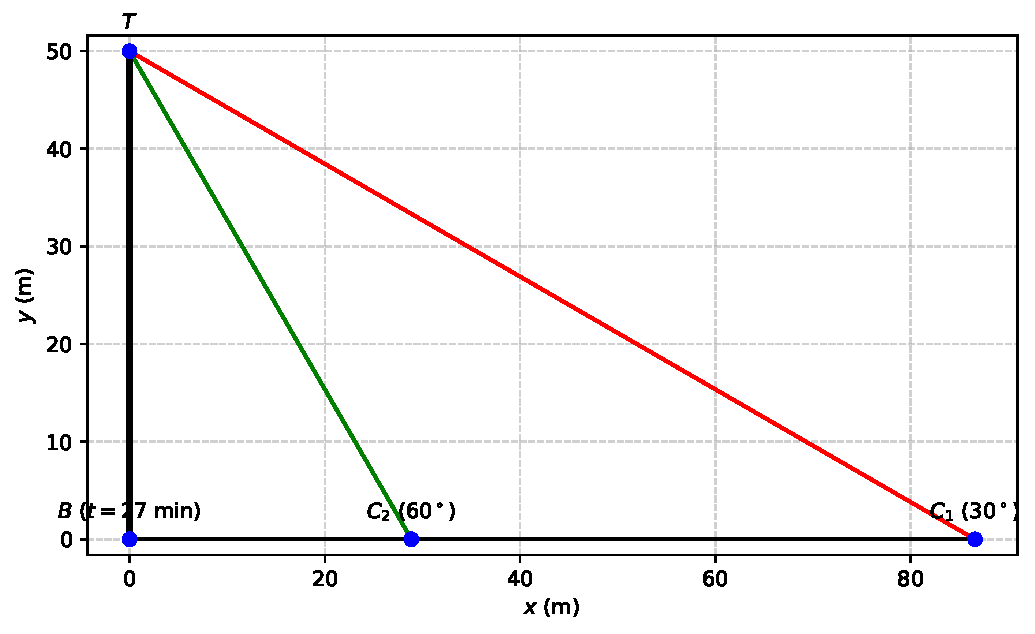
\includegraphics[width=0.70\linewidth]{figs/cbXq35.pdf}
    \caption{Car approaching the tower: angles of depression $30^{\circ}$ and $60^{\circ}$}
    \label{fig:EE26BTECH11218-cb_q35}
\end{figure}
\end{enumerate}
